\subsection{Đề 2}
\caulc
\Opensolutionfile{ans}[ans/ans-1-CTST-DE2]
\begin{ex}%[1D1H5-3]
Tất cả nghiệm của phương trình $2\cos x+1=0$ là
\choice
{$x=\pm\dfrac{2\pi}{3}+k\pi$, $k \in \mathbb{Z}$}
{$x=\pm\dfrac{\pi}{3}+k\pi$, $k \in \mathbb{Z}$}
{$x=\pm\dfrac{\pi}{3}+k2\pi$, $k \in \mathbb{Z}$}
{\True $x=\pm\dfrac{2\pi}{3}+k2\pi$, $k \in \mathbb{Z}$}
\loigiai{
	Ta có $2\cos x+1=0$ $\Leftrightarrow\cos x=-\dfrac{1}{2}\Leftrightarrow\cos x=\cos\dfrac{2\pi}{3} \Leftrightarrow x=\pm\dfrac{2\pi}{3}+k2\pi$, $k \in \mathbb{Z}$.
}
\end{ex}

\begin{ex}%[1D2H3-5]
Tìm tất cả giá trị của $x$ để ba số $2x$, $7x+6$, $6 x^2-24$ theo thứ tự đó lập thành một cấp số nhân.
\choice
{$x=4$}
{$x=5$}
{\True $x=6$}
{$x=7$}
\loigiai{	
	Áp dụng tính chất của cấp số nhân, ta có
	$$
	\begin{aligned}
		& (2 x)\left(6 x^2-24\right)=(7 x+6)^2 \\
		& \Leftrightarrow 12 x^3-48 x=49 x^2+84 x+36 \\
		& \Leftrightarrow 12 x^3-49 x^2-132 x-36=0
	\end{aligned}
	$$
	Vì lấy $x$ nguyên nên nhận $x=6$.
}
\end{ex}

\begin{ex}%[1D3N1-2]
Tính giới hạn $\displaystyle\lim\dfrac{2n-1}{n-1}$.
\choice
{$-2$}
{$1$}
{\True $2$}
{$-1$}
\loigiai{
	Ta có $\lim\dfrac{2n-1}{n-1}=\lim\dfrac{2-\dfrac{1}{n}}{1-\dfrac{1}{n}} = 2$.
}
\end{ex}

\begin{ex}%[1D3N2-2]
	Cho hai hàm số $f(x)$, $g(x)$ có giới hạn hữu hạn tại $x=a$ đồng thời thỏa mãn các điều kiện\break $\lim\limits_{x\to a} [2f(x)-3g(x)]=3$ và $\lim\limits_{x\to a} [f(x)+6g(x)]=4$. Tính giới hạn $L=\lim\limits_{x\to a} [2(f(x)+g(x))]$.
	\choice
	{$L=\dfrac{7}{3}$}
	{$L=\dfrac{7}{6}$}
	{\True $L=\dfrac{14}{3}$}
	{$L=7$}
	\loigiai
	{
		Ta có
		\[\heva{&\lim\limits_{x\to a} [2f(x)-3g(x)]=3 \\& \lim\limits_{x\to a} [f(x)+6g(x)]=4}\Leftrightarrow \heva{&2\lim\limits_{x\to a} f(x)-3\lim\limits_{x\to a} g(x)=3 \\& \lim\limits_{x\to a}f(x)+6\lim\limits_{x\to a}g(x) = 4 }\Leftrightarrow \heva{&\lim\limits_{x\to a}f(x)= 2\\& \lim\limits_{x\to a}g(x)= \dfrac{1}{3}. }\]
		Vậy $L=\lim\limits_{x\to a} [2(f(x)+g(x))]=2\left[\lim\limits_{x\to a}f(x)+\lim\limits_{x\to a}g(x)\right] = 2\cdot\left(2+\dfrac{1}{3}\right) = \dfrac{14}{3}$.
}
\end{ex}

\begin{ex}%[1D3N3-3]
Khẳng định nào đúng?
\choice
{\True Hàm số $f(x)=\dfrac{x+1}{\sqrt{x^2+1}}$ liên tục trên $\mathbb{R}$}
{Hàm số $f(x)=\dfrac{x+1}{x-1}$ liên tục trên $\mathbb{R}$}
{Hàm số $f(x)=\dfrac{x+1}{\sqrt{x-1}}$ liên tục trên $\mathbb{R}$}
{Hàm số $f(x)=\dfrac{\sqrt{x+1}}{x-1}$ liên tục trên $\mathbb{R}$}
\loigiai{
	Hàm số $f(x)=\dfrac{x+1}{\sqrt{x^2+1}}$ là hàm phân thức có tập xác định là $\mathbb{R}$ nên liên tục trên $\mathbb{R}$.
}
\end{ex}

\begin{ex}%[1D3N3-3]
Cho hàm số $f(x)=\heva{&3 x+2 & \text{khi } x<-1 \\& x^2-1 & \text{khi } x \geq-1}$. Khẳng định nào sau đây đúng?
\choice
{$f(x)$ liên tục trên $\mathbb{R}$}
{$f(x)$ liên tục trên $(-\infty;-1]$}
{\True $f(x)$ liên tục trên $[-1;+\infty)$}
{$f(x)$ liên tục tại $x=-1$}
\loigiai{
	Hàm số xác định trên $\mathbb{R}$.\\
	Ta có $f(-1)=0; \lim\limits_{x \to-1^{+}} f(x)=\lim\limits_{x \to-1^{+}}\left(x^2-1\right)=0, \lim\limits_{x \to-1^{-}} f(x)=\lim\limits_{x \to-1^{-}}(3 x+2)=-1$.\\
	Suy ra $f(-1)=\lim\limits_{x \to-1^{+}} f(x) \neq \lim\limits_{x \to-1^{-}} f(x)$.\\
	Vậy hàm số đã cho liên tục trên nửa khoảng $[-1;+\infty)$ và khoảng $(-\infty;-1)$.	
}
\end{ex}

\begin{ex}%[1H4N4-2]
Cho hình hộp $ABCD.A'B'C'D'$. Mặt phẳng $(AB'D')$ song song với mặt phẳng nào sau đây?
\choice
{$(BA'C')$}
{\True $(C'BD)$}
{$(BDA')$}
{$(ACD')$}
\loigiai{
\immini{
Ta có $\heva{&B'D'\parallel BD\\&BD\subset (C'BD)}\Rightarrow B'D'\parallel (C'BD)$.\\
Mặt khác $\heva{&AB'\parallel C'D\\&C'D\subset (C'BD)}\Rightarrow AB'\parallel (C'BD)$.\\
Mà $\heva{&B'D',AB'\subset (AB'D')\\&B'D'\cap AB'=B'}$.\\
Vậy $(AB'D')\parallel ((C'BD))$.
}
{\begin{tikzpicture}[scale=1,line join=round,font=\footnotesize ,line cap=round,>=stealth,thick]
	\def\a{3.5}
	\def\h{4.5}
	\path 	(0:0) coordinate (A)
	++(0:\a) coordinate (D)
	++(-130:\a/2) coordinate (C)
	($(A)+(C)-(D)$) coordinate (B)	
	($(A)!0.45!(C)$) coordinate (H)
	($(H)+(90:\h)$) coordinate (A')
	($(A')+(C)-(A)$) coordinate (C')
	($(C')+(B)-(C)$) coordinate (B')
	($(A')+(D)-(A)$) coordinate (D');
	\draw[dashed,thick] 	(B)--(A)--(D)	(A)--(A') (D')--(A)--(B') (B)--(D);
	\draw[thick] (B')--(D')	(C)--(C') 	(D)--(D') 	(B)--(B')  (B)--(C)--(D) (A')--(B')--(C')--(D')--cycle (D)--(C')--(B);
	\foreach \x/\g in {A/180,B/180,C/0,D/0,A'/180,B'/180,C'/0,D'/0}
	\fill[black] 	(\x) circle (1pt)
	($(\g:4mm)+(\x)$) node {$\x$};
%	\draw pic[draw,angle radius=2mm]{right angle=A'--H--C};%Theo chiều dương		
\end{tikzpicture}}
}
\end{ex}

\begin{ex}%[1H4N6-1]
Một tấm bảng nghiêng so với mặt đất được chiếu lên bức tường thẳng đứng bằng ánh sáng chiếu xiên từ một nguồn sáng xa. Hình ảnh của tấm bảng trên bức tường sẽ là
\choice
{Một đường thẳng}
{Một hình tam giác}
{\True Một hình chữ nhật}
{Một hình tròn}
\loigiai{
\begin{itemize}
	\item Khi ánh sáng chiếu xiên từ một nguồn sáng xa, các tia chiếu song song sẽ chiếu hình ảnh của tấm bảng nghiêng lên bức tường thẳng đứng.
	\item Tấm bảng nghiêng có hình chữ nhật, khi chiếu song song lên bức tường, hình ảnh của nó vẫn giữ nguyên dạng là hình chữ nhật, nhưng có thể bị biến dạng theo góc chiếu.
	\item Tuy nhiên, do tính chất của phép chiếu song song, các cạnh của hình chữ nhật sẽ vẫn song song và duy trì hình dạng cơ bản của nó.
\end{itemize}
	Vậy hình ảnh của tấm bảng trên bức tường sẽ là \lq\lq Một hình chữ nhật\rq\rq.
}
\end{ex}

\begin{ex}%[1D5N1-3]
Doanh thu bán hàng trong $20$ ngày được lựa chọn ngẫu nhiên của một của hàng được ghi lại ở bảng sau (đơn vị: triệu đồng):
\begin{center}
	\begin{tabular}{|c|c|c|c|c|c|}
		\hline
		Doanh thu		&	$\left[5;7\right)$ & $\left[7;9\right)$ &$\left[9;11\right)$ &$\left[11;13\right)$ &$\left[13;15\right)$ \\
		\hline
		Số ngày		& $2$ &$7$ &$7$ &$3$ &$1$ \\
		\hline
	\end{tabular}
\end{center}
Số trung bình của mẫu số liệu trên thuộc khoảng nào trong các khoảng dưới đây?
\choice
{$\left[7;9\right)$}
{\True $\left[9;11\right)$}
{$\left[11;13\right)$}
{$\left[13;15\right)$}
\loigiai{
	Bảng tần số ghép nhóm theo giá trị đại diện là
	\begin{center}
		\begin{tabular}{|c|c|c|c|c|c|}
			\hline
			Doanh thu		&	$\left[5;7\right)$ & $\left[7;9\right)$ &$\left[9;11\right)$ &$\left[11;13\right)$ &$\left[13;15\right)$ \\
			\hline
			Giá trị đại diện		& $6$ &$8$ &$10$ &$12$ &$14$ \\
			\hline
			Số học sinh		& $2$ &$7$ &$7$ &$3$ &$1$ \\
			\hline
		\end{tabular}
	\end{center}
	Số trung bình $\overline{x}=\dfrac{2\cdot 6+7\cdot 8+7\cdot 10+3\cdot 12+1\cdot 14}{20}=9{,}4$.
}
\end{ex}

\begin{ex}%[1D5N1-4]
Khảo sát thời gian tập thể dục của một số học sinh khối $11$ thu được mẫu số liệu ghép nhóm sau:
\begin{center}
	\begin{tabular}{|c|c|c|c|c|}
		\hline
		Thời gian (Phút)		&	$\left[0;20\right)$ & $\left[20;40\right)$ &$\left[40;60\right)$ &$\left[60;80\right)$  \\
		\hline
		Số học sinh		& $5$ &$9$ &$12$ &$10$  \\
		\hline
	\end{tabular}
\end{center}
Nhóm chứa mốt của mẫu số liệu trên là
\choice
{$[0;20)$}
{$[20;40)$}
{\True $[40;60)$}
{$[60;80)$}
\loigiai{
Nhóm chứa mốt là nhóm có tần số lớn nhất.\\
Do đó nhóm chứa mốt là nhóm $[40;60)$ có tần số là $12$.
}
\end{ex}

\begin{ex}%[1D5N2-2]
Doanh thu bán hàng trong $20$ ngày được lựa chọn ngẫu nhiên của một của hàng được ghi lại ở bảng sau (đơn vị: triệu đồng):
\begin{center}
	\begin{tabular}{|c|c|c|c|c|c|}
		\hline
		Doanh thu		&	$\left[5;7\right)$ & $\left[7;9\right)$ &$\left[9;11\right)$ &$\left[11;13\right)$ &$\left[13;15\right)$ \\
		\hline
		Số ngày		& $2$ &$7$ &$7$ &$3$ &$1$ \\
		\hline
	\end{tabular}
\end{center}
Trung vị của mẫu số liệu trên thuộc khoảng nào trong các khoảng dưới đây?
\choice
{$\left[7;9\right)$}
{\True $\left[9;11\right)$}
{$\left[11;13\right)$}
{$\left[13;15\right)$}
\loigiai{
	Gọi $x_1,x_2,\ldots,x_{20}$ là doanh thu bán hàng trong $20$ ngày xếp theo thứ tự không giảm.\\
	Khi đó $x_1,x_2\in \left[5;7\right)$; $x_3,\ldots, x_9\in \left[7;9\right)$; $x_{10},\ldots, x_{16}\in \left[9;11\right)$; $x_{17},\ldots, x_{19}\in \left[11;13\right)$; $x_{20}\in \left[13;15\right)$.\\
	Do đó, trung vị của mẫu số liệu thuộc nhóm $\left[9;11\right)$.
}
\end{ex}

\begin{ex}%[1D5N2-3]
Khảo sát thời gian tập thể dục của một số học sinh khối 11 thu được mẫu số liệu ghép nhóm sau:
\begin{center}
	\begin{tabular}{|c|c|c|c|c|c|}
		\hline
		Thời gian (Phút)		&	$\left[0;20\right)$ & $\left[20;40\right)$ &$\left[40;60\right)$ &$\left[60;80\right)$ &$\left[80;100\right)$ \\
		\hline
		Số học sinh		& $5$ &$9$ &$12$ &$10$ &$6$ \\
		\hline
	\end{tabular}
\end{center}
Nhóm chứa tứ phân vị thứ ba của mẫu số liệu trên là
\choice
{$\left[40;60\right)$}
{$\left[20;40\right)$}
{\True $\left[60;80\right)$}
{$\left[80;100\right)$}
\loigiai{
	Ta có $n=42$ nên tứ phân vị thứ ba của mẫu số liệu trên là $Q_3=x_{33}$.\\
	Mà $x_{33}\in \left[60;80\right)$.\\
	Vậy nhóm chứa tứ phân vị thứ ba của mẫu số liệu trên là nhóm $\left[60;80\right)$.
}
\end{ex}
\Closesolutionfile{ans}
\indapan{6}{ans/ans-1-CTST-DE2}
\cauds
\Opensolutionfile{ans}[ans/ans-1-CTST-DE2-DS]
\begin{ex}%[1H4N4-1]
Cho hình chóp $S.ABCD$ có $ABCD$ là hình thang với $BC$ là đáy bé. 
\choiceTF
{\True Giao tuyến của $2$ mặt phẳng $(SAD)$ và $(SAB)$ là $SA$}
{Giao tuyến của $2$ mặt phẳng $(SAD)$ và $(SBC)$ là đường thẳng $SO$, với $O=AC \cap BD$}
{\True Giao tuyến của $2$ mặt phẳng $(SAC)$ và $(SBD)$ là đường thẳng $SO$, với $O=AC \cap BD$}
{\True Giao điểm của $CD$ với mặt phẳng $(SAB)$ là $I$ với $I=CD \cap AB$}
\loigiai{
	\begin{center}
		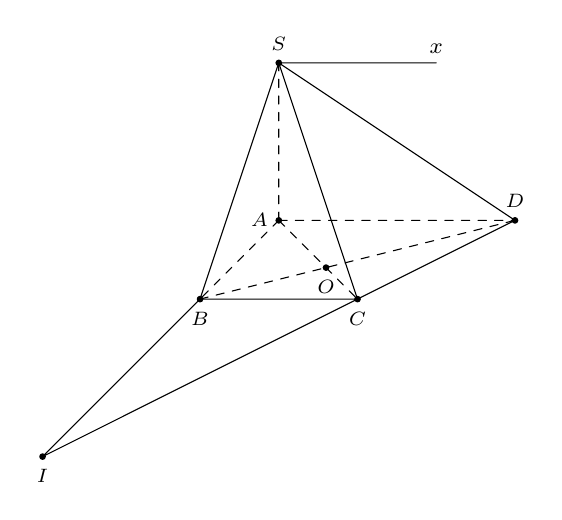
\begin{tikzpicture}[line join = round, line cap = round,>=stealth,font=\footnotesize,scale=1]
			\foreach \x/\y/\t in {0/0/A,3/0/D,-1/-1/B,1/-1/C,0/2/S,2/2/x}{
				\path (\x,\y) coordinate (\t);
			}
			\path 
			(intersection of A--C and B--D) coordinate (O)
			(intersection of D--C and B--A) coordinate (I)
			;
			\draw[dashed] (A)--(S) (A)--(B) (A)--(D) (A)--(C) (B)--(D);
			\draw (S)--(B) (S)--(C) (S)--(D) (B)--(C) (C)--(D) (S)--(x)node[above]{$x$} (B)--(I)--(C);
			\foreach \t/\g in {A/180,B/-90,C/-90,D/90,S/90,O/-90,I/-90}{
				\draw[fill=black] (\t) circle (1pt) node[shift={(\g:7pt)},font=\scriptsize]{$ \t $};
			}
		\end{tikzpicture}	
	\end{center}
	\begin{itemchoice}
		\itemch{\bf Đúng.}\\
		Ta có giao tuyến của $2$ mặt phẳng $(SAD)$ và $(SAB)$ là $SA$.
		\itemch{\bf Sai.}\\
		Ta có $\heva{& AD\in (SAD) \\ & BC\in (SBC)\\ & S\in (SAD)\cap (SBC)\\ & AD\parallel BC}\Rightarrow (SBC)\cap (SAD)=Sx\parallel AD\parallel BC$.
		\itemch{\bf Đúng.}\\
		Ta có giao tuyến của $2$ mặt phẳng $(SAC)$ và $(SBD)$ là đường thẳng $SO$, với $O=AC \cap BD$.
		\itemch{\bf Đúng.}\\
		Vì $I=CD \cap AB$ nên giao điểm của $CD$ với mặt phẳng $(SAB)$ là $I$.
	\end{itemchoice}	
	}
\end{ex}

\begin{ex}%[1H4H1-3]
Cho hình chóp $S.ABCD$ có $ABCD$ là hình thang với hai cạnh đáy là $AD$ và $BC$, đáy lớn là $AD$. Gọi $M$, $N$ lần lượt là trung điểm của $SA$ và $SD$.
\choiceTF
{\True $MN$ song song $BC$}
{\True Giao tuyến của $(SAD)$ và $(SBC)$ là  đường thẳng qua $S$ và song song với $AD$}
{\True Giao điểm của $SB$ và $(MCD)$ là $F=SB\cap ME$}
{Giao tuyến của $(SAB)$ và $(SCD)$ là  đường thẳng qua $S$ và song song với $AB$}
\loigiai{
	\begin{center}
		\begin{tikzpicture}[scale=1, font=\footnotesize, line join=round, line cap=round,>=stealth]
			\path (0,0)coordinate (B) (3,0) coordinate (C) (1,1) coordinate (A) ($(A)+(C)-(B)+(1.5,0)$) coordinate (D) (0.3,2.7) coordinate (h) ($(A)+(h)$) coordinate (S) ($(S)!0.5!(A)$) coordinate (M) ($(S)!0.5!(D)$) coordinate (N) (intersection of A--B and C--D) coordinate (E) (intersection of S--B and M--E) coordinate (F);
			\draw (S)--(F)--(C)--(D)--cycle (S)--(C)--(F)--(E)--(C);
			\draw[shorten <=-1cm,shorten >=-1cm] (S)--+(2.5,0) node[pos=1.2, above]{$x$};
			\draw[dashed] (S)--(A)--(B)--(F)--(M)--(D)--(A) (E)--(B)--(C)--(M)--(N) ;
			\foreach \p/\g in {A/150,B/-60,C/-60, D/0, S/90,M/45,N/30,E/-90,F/150} \fill[black] (\p) circle(1pt)+(\g:0.3) node{$\p$};
		\end{tikzpicture}
	\end{center}
		\begin{itemchoice}
		\itemch{\bf Đúng.}\\
		Ta có $MN$ là đường trung bình của tam giác $SAD$ nên $MN\parallel AD$.\\
		Vì $ABCD$ là hình thang nên $BC\parallel AD$.\\
		Suy ra $MN\parallel BC$.
		\itemch{\bf Đúng.}\\
		Ta có $\heva{&S\in (SAD)\cap (SBC)\\ & AD\parallel BC \\ & AD\subset (SAD)\\ & BC\subset (SBC) }\Rightarrow (SAD)\cap (SBC)=Sx$, trong đó $Sx\parallel AD\parallel BC$
		\itemch{\bf Đúng.}\\
		Ta có $SB\subset (SAB)$.\\
		Trong $(ABCD)$ gọi $E=AB\cap CD$.\\
		Khi đó $\heva{& E\in AB, AB\subset (SAB) \\ & E\in CD, CD\subset (MCD)}\Rightarrow E\in (SAB)\cap (MCD)$.\\
		Dễ thấy $M\in (SAB)\cap (MCD)$.\\
		Do đó, $(SAB)\cap (MCD)=ME$.\\
		Trong $(SAB)$, gọi $F=SB\cap ME$.\\
		Vậy $F=SB\cap (MCD)$.
		\itemch{\bf Sai.}\\
		Ta có $S\in (SAB)\cap (SCD)$.\\
		$\heva{&E\in AB\\&AB\subset (SAB)}\Rightarrow E\in (SAB)$.\\
		$\heva{&E\in CD\\&CD\subset (SCD)}\Rightarrow E\in (SCD)$.\\
		Suy ra  $E\in (SAB)\cap (SCD)$.\\
		Vậy $(SAB)\cap (SCD)=SE$.		
	\end{itemchoice}
}
\end{ex}

\begin{ex}%[1H4H3-2]
Cho tứ diện $ABCD$ có điểm $G$ là trọng tâm tam giác $ABD$ và điểm $M$ thuộc cạnh $BC$ sao cho $MB=2MC$. Khẳng định nào dưới đây là đúng?
\choiceTF
{$MG $ cắt $AC$}
{$MG \parallel AB $}
{\True $MG \parallel (ACD) $}
{$(BMG)\cap (ACD)=MG$}
\loigiai{
	\begin{center}
		\begin{tikzpicture}[scale=.7,>=stealth, font=\footnotesize, line join=round, line cap=round]
			
			\foreach \x/\y/\t in {0/0/B,1.3/-1.6/C,4.5/0/D,1/3.5/A}{
				\path (\x,\y) coordinate (\t);
			}
			\path
			(barycentric cs:A=1,B=1,D=1) coordinate (G)
			($(B)!2/3!(C)$) coordinate (M)
			($(A)!.5!(D)$) coordinate (I)
			;
			\draw[dashed] (D)--(B)--(I) (M)--(G);
			\draw (A)--(B)--(C)--(D)--(A)--(C)--(I);
			\foreach \t/\g in {A/90,B/180,C/-90,D/0,G/90,M/190,I/60}{
				\draw[fill=black] (\t) circle (1pt) node[shift={(\g:7pt)},font=\scriptsize]{$ \t $};
			}
		\end{tikzpicture}	
	\end{center}
		\begin{itemchoice}
		\itemch{\bf Sai.}\\
		Vì $MG$ và $AC$ không đồng phẳng nên $MG$ không cắt $AC$.
		\itemch{\bf Sai.}\\
		Vì $MG$ và $AB$ không đồng phẳng nên $MG$ không song $AB$.
		\itemch{\bf Đúng.}\\
		Gọi $I$ là trung điểm $AD$. Vì $G$ là trọng tâm tam giác $ABD$ nên $\dfrac{BG}{BI}=\dfrac{2}{3}$.\\
		Lại có $\dfrac{BM}{BC}=\dfrac{2}{3}$ nên $MG\parallel CI$ (định lí Ta-lét đảo).\\
		Mà $CI \subset (ACD)$ nên $MG\parallel (ACD)$.
		\itemch{\bf Sai.}\\		
		Ta có $(BMG)\equiv (BIC)$ nên $(BMG)\cap (ACD)=CI$.
	\end{itemchoice}
}
\end{ex}

\begin{ex}%[1D5H2-3]
Trong một đề tài nghiên cứu về bệnh A, người ta ghi lại lại tuổi của bệnh nhân mắc bệnh này, số liệu thông kê được trình bày trong bảng sau
\begin{center}
	\begin{tabular}{|c|c|c|c|c|c|}
		\hline
		Độ tuổi &	$\left[15;25\right)$ & $\left[25;35\right)$ &$\left[35;45\right)$ &$\left[45;55\right)$ &$\left[55;65\right)$ \\
		\hline
		Số bệnh nhân		& $10$ &$12$ &$14$ &$9$ &$5$ \\
		\hline
	\end{tabular}
\end{center}
Khi đó
\choiceTF
{\True Cỡ mẫu là $n=50$}
{Trung vị của mẫu số liệu  thuộc nhóm $\left[25;35\right)$}
{\True Trung vị của mẫu số liệu gần bằng $37{,}14$}
{\True Khoảng tứ phân vị gần bằng $19$}
\loigiai{
\begin{itemchoice}
\itemch{\bf Đúng.}\\
	Cỡ mẫu là $n=50$.
\itemch{\bf Sai}\\
	Gọi $x_1,x_2,\ldots,x_{50}$ là độ tuổi của $50$ bệnh nhân và giả sử dãy này được sắp xếp theo thứ tự tăng dần.\\
	Khi đó trung vị của mẫu số liệu là $\dfrac{x_{25}+x_{26}}{2}$. Do $x_{25},x_{26}$ thuộc nhóm $\left[35;45\right)$ nên nhóm này chứa trung vị.
\itemch{\bf Đúng.}\\
	Gọi $x_1,x_2,\ldots,x_{50}$ là độ tuổi của $50$ bệnh nhân và giả sử dãy này được sắp xếp theo thứ tự tăng dần.\\
	Khi đó trung vị của mẫu số liệu là $\dfrac{x_{25}+x_{26}}{2}$. Do $x_{25},x_{26}$ thuộc nhóm $\left[35;45\right)$ nên nhóm này chứa trung vị.\\
	Ta xác định được $n=50$; $p=3$; $m_3=14$; $m_1+m_2=22$, $a_3=35$, $a_4=45$.\\
	Vậy trung vị của mẫu số liệu ghép nhóm là $M_e=35+\dfrac{\dfrac{50}{2}-22}{14}\cdot (45-35)\approx 37{,}14$.
\itemch{\bf Đúng}\\
Cỡ mẫu $n=50$ nên tứ phân vị thứ nhất là $Q_1=\dfrac{x_{11}+x_{13}}{2}\in [25;35)$.\\
Do đó $Q_1=25+\dfrac{\dfrac{50}{4}-10}{12}\cdot 10=27{,}08$.\\
Tứ phân vị thứ ba là $Q_1=\dfrac{x_{36}+x_{38}}{2}\in [35;45)$.\\
Do đó $Q_3=35+\dfrac{\dfrac{3\cdot 50}{4}-22}{14}\cdot 10=46{,}07$.\\
Vậy $Q_3-Q_1\approx 46{,}07-27{,}08\approx 19$.
\end{itemchoice}
}
\end{ex}
\Closesolutionfile{ans}
\indapan{2}{ans/ans-1-CTST-DE2-DS}
\caukq
\Opensolutionfile{ans}[ans/ans-1-CTST-DE2-KQ]
\begin{ex}%[1D1V5-3]
Hằng ngày mực nước của con kênh lên xuống theo thủy triều. Độ sâu $h$ (mét) của mực nước trong kênh được tính tại thời điểm $t$ (giờ) trong một ngày ($t > 0$) bởi công thức $h=4\sin (\dfrac{\pi t}{8}+\dfrac{5\pi}{8})+16$. Mực nước của kênh cao nhất khi $t$ bằng bao nhiêu?
\shortans[6]{$15$}
\loigiai{
Mực nước của kênh cao nhất khi $h$ lớn nhất
$$ \sin (\dfrac{\pi t}{8}+\dfrac{5\pi}{8})=1\Leftrightarrow \dfrac{\pi}{8}t+\dfrac{5\pi}{8}=\dfrac{\pi}{2}+k2\pi \Leftrightarrow t=-1+16k, k\in\mathbb{Z}.$$
Với $0 < t\le 24$ suy ra $0 <-1+16k\le 24\Leftrightarrow \dfrac{1}{16} < k\le \dfrac{25}{16}$.\\
Do $k\in \mathbb{Z}$ nên $k=1$ thỏa mãn. Khi $k=1$ thì $t=15$ h.
}
\end{ex}

\begin{ex}%[1D2V2-7]
Một rạp hát có $18$ hàng ghế xếp theo hình quạt. Hàng thứ nhất có $16$ ghế, hàng thứ hai có $20$ ghế, hàng thứ ba có $24$ ghế, $\ldots$ cứ thế cho đến hàng cuối cùng. Hỏi tổng số ghế có trong rạp là bao nhiêu?
\shortans[6]{$900$}
\loigiai{
Gọi số ghế ở hàng thứ $n$ là $u_n$.\\
Ta có $u_1=16$; $u_2=20$, $u_3=24$.\\
Nhận xét dãy số $(u_n)$ là cấp số cộng có $u_1=16$, công sai $d=u_2-u_1=20-16=4$.\\
Khi đó
\begin{equation*}
	S_{18}=\dfrac{n\left[2u_1+(n-1)d\right]}{2}=\dfrac{18\cdot(2\cdot16+17\cdot4)}{2}=900.
\end{equation*}
Vậy tổng số ghế trong rạp là $900$ ghế.
}
\end{ex}

\begin{ex}%[1D2V3-8]
Một du khách vào chuồng đua ngựa đặt cược, lần đầu đặt $50\,000$ đồng, mỗi lần sau đặt gấp đôi lần cọc trước. Người đó thua $10$ lần liên tiếp và thắng ở lần thứ $11$. Hỏi du khách trên thắng hay thua bao nhiêu tiền (đơn vị nghìn đồng)?
\shortans[6]{$50$}
\loigiai{
Số lần đặt cược tạo thành một cấp số nhân với số hạng đầu $u_1=50\,000$ và công bội $q=2$.\\
Du khách thua trong $10$ lần liên tiếp nên tổng số tiền thua là
$${S_{10}}=u_1+u_2+\cdots+{u_{10}}=u_1\cdot\dfrac{1-{q^{10}}}{1-q}=50\,000\cdot\dfrac{1-2^{10}}{1-2}=51\,150\,000.$$
Số tiền du khách thắng trong lần thứ $11$ là $u_{11}=u_1\cdot q^{10}=50000\cdot2^{10}=51\,200\,000$.\\
Ta có $u_{11}-S_{10}=51200000-51150000=50\,000$ nên du khách đó thắng $50\,000$ đồng.
}
\end{ex}

\begin{ex}%[1D3V3-3]
Cho hàm số $f(x)=\heva{&\dfrac{\sqrt[3]{x+7}-\sqrt{3 x+1}}{x-1}, & \text{khi } x \neq 1 \\& a x, & \text{khi } x=1}$. Tìm giá trị của $a$ để hàm số liên tục tại $x_0=1$ (làm tròn kết quả đến hàng phần mười).
\shortans[6]{$-0{,}7$}
\loigiai{
Ta có $f(1)=a$.
{\allowdisplaybreaks
	\begin{eqnarray*}
		\lim\limits_{x \to 1} \dfrac{\sqrt[3]{x+7}-\sqrt{3 x+1}}{x-1}&=&\lim\limits_{x \to 1} \dfrac{\sqrt[3]{x+7}-2}{x-1}+\lim\limits_{x \to 1} \dfrac{2-\sqrt{3 x+1}}{x-1}\\
		&=&\lim\limits_{x \to 1} \dfrac{1}{\sqrt[3]{(x+7)^2}+2 \sqrt[3]{x+7}+4}+\lim\limits_{x \to 1} \dfrac{-3}{2+\sqrt{3 x+1}} \\
		&=&\dfrac{1}{12}-\dfrac{3}{4}=-\dfrac{2}{3}.
\end{eqnarray*}}
Để hàm số liên tục tại $x=1$ thì $a=-\dfrac{2}{3}\approx -0{,}7$.
}
\end{ex}

\begin{ex}%[1H4V6-5]
Cho hình chóp $S.ABCD$, đáy $ABCD$ là hình bình hành có $O$ là giao điểm của của $AC$ và $BD$, $AC=6$, $BD=8$; tam giác $SBD$ là tam giác đều. Gọi $I$ là điểm nằm trên doạn thẳng $AC$ sao cho $AI=x\,(0<x<3)$, $(P)$ là mặt phẳng đi qua diểm $I$ và song song với mặt phẳng $(SBD)$. Diện tích của hình tạo bởi các đoạn giao tuyến của mặt phẳng $(P)$ với các mặt của hình chóp $S.ABCD$ bằng $\dfrac{m^2x^2\sqrt{3}}{n^2}$. Tính giá trị của biểu thức $P=m^2+n^2$.
\shortans[6]{$73$}
\loigiai{
\begin{center}
	\begin{tikzpicture}[scale=1,line join=round,font=\footnotesize ,line cap=round,thick]
		\coordinate (A) at (0,0);
		\coordinate (B) at (-2,-2);
		\coordinate (D) at (5,0);
		\coordinate (C) at ($(B)+(D)-(A)$);
		\coordinate (S) at ($(A)+(1,4)$);
	\path ($(A)!0.5!(C)$) coordinate (O) ;	
	\path ($(A)!0.4!(O)$) coordinate (I) ;
	\path ($(A)!0.4!(B)$) coordinate (M) ;
	\path ($(A)!0.4!(D)$) coordinate (N) ;
	\path ($(S)!0.6!(A)$) coordinate (J) ;
		\draw(S)--(B) (S)--(C) (S)--(D) (B)--(C)--(D);
		\draw[dashed,thin](S)--(A) (A)--(B) (A)--(D)(A)--(C)(B)--(D) (M)--(N)--(J)--cycle;
		\foreach \i/\g in {S/90,A/45,B/-90,C/-90,D/0,O/-90,M/180,N/-90,J/45,I/-90}{\draw[fill=black](\i) circle (1pt) ($(\i)+(\g:3mm)$) node[scale=1]{$\i$};}
	\end{tikzpicture}
\end{center}	
Trong mặt phẳng $(ABCD)$, kẻ $MN$ đi qua $I$ và $MN\parallel BD\,(M\in AB, N\in AD)$.\\
Trong mặt phẳng $(SAD)$, kẻ $IJ\parallel SD\,(J\in SA)$.\\
Trong mặt phẳng $(SAB)$ nối $JM$.\\
Khi đó $(P)\cap (SAB)=JM$, $(P)\cap (SAD)=JN$, $(P)\cap (ABCD)=MN$.\\
Do đó các đoạn giao tuyến của mặt phẳng $(P)$ với các mặt của hình chóp $S.ABCD$ tạo thành tam giác $JMN$.\\
Ta có $\triangle JMN\backsim \triangle SBD$ nên $\triangle JMN$ là tam giác đều.\\
Khi đó $MN\parallel BD$, suy ra $\dfrac{MN}{BD}=\dfrac{AI}{AO}=\dfrac{x}{3}\Rightarrow MN=\dfrac{8x}{3}$\\
$\Rightarrow S_{\triangle JMN}=\dfrac{8^2x^2\sqrt{3}}{3^2}\Rightarrow m^2=8^2$ và $n^2=3^2$.\\
Vậy $P=m^2+n^2=8^2+3^2=73$.

}
\end{ex}

\begin{ex}%[1D5V2-3]
Phỏng vấn một số học sinh khối $11$ về thời gian (giờ) ngủ của một buổi tối, thu được bảng số
liệu sau:
\begin{center}
	\begin{tabular}{|c|c|c|c|c|c|}
		\hline
		Thời gian (Giờ)		&	$\left[4;5\right)$ & $\left[5;6\right)$ &$\left[6;7\right)$ &$\left[7;8\right)$ &$\left[8;9\right)$ \\
		\hline
		Số lượng		& $6$ &$12$ &$13$ &$10$ &$3$ \\
		\hline
	\end{tabular}
\end{center}
Hãy cho biết $75\%$ học sinh khối $11$ ngủ nhiều nhất bao nhiêu giờ?
\shortans[6]{$7{,}2$}
\loigiai{
Cỡ mẫu là $n=44$.\\
Tứ phân vị thứ hai $Q_2$ là giá trị của $\dfrac{x_{22}+x_{23}}{2}$.\\
Tứ phân vị thứ nhất $Q_1$ là giá trị của $\dfrac{x_{11}+x_{12}}{2}$.\\
Tứ phân vị thứ ba $Q_2$ là giá trị của $\dfrac{x_{33}+x_{34}}{2}$.\\
Do $x_{33};x_{34}$ thuộc nhóm $\left[7;8\right)$ nên nhóm này chứa $Q_3$.\\
Ta xác định được $n=44$; $p=4$; $m_4=10$; $m_1+m_2+m_3=31$, $a_5=8$, $a_4=7$.\\
Vậy $Q_3=7+\dfrac{33-31}{10}\cdot (8-7)=7{,}2$.\\
Vậy tứ phân vị thứ ba nên $75\%$ học sinh khối $11$ ngủ nhiều nhất là $7{,}2$ giờ.
}
\end{ex}
\Closesolutionfile{ans}
\indapan{6}{ans/ans-1-CTST-DE2-KQ}